\section{实验原理}

\subsection{IMU增量数据与单位换算}
\begin{table}[htbp]\centering\small
\caption{处理采用的常数与计数系数}\label{tab:constants}
\begin{tabularx}{\textwidth}{p{4.5cm}Y}\toprule
项目&取值与说明\\\midrule
纬度$L$、椭球高$h$&$30.531651244^\circ$（北纬），$28.2134$~m\\
重力$g$&$9.7936174$~m/s$^2$\\
地球自转$\Omega$&$7.292115\times10^{-5}$~rad/s\\
采样率与增量时长&$f_s=200$~Hz，$\Delta t=0.005$~s\\
XW-GI7681加速度计$q_a$&$0.05/2^{15}=1.52587890625\times10^{-6}$~(m/s)/LSB\\
XW-GI7681陀螺$q_g$&$[0.1/(3600\times256)]\pi/180=1.89380344\times10^{-9}$~rad/LSB\\
100C加速度计/陀螺&$2.0\times10^{-8}$~(m/s)/LSB；$1.0\times10^{-9}$~rad/LSB\\\bottomrule
\end{tabularx}\end{table}

先按分号分离消息头和数据体，再分离星号后的校验值。RAWIMUSA数据体含9个字段；RAWIMUXA多出IMU信息和型号两个字段，含11个字段。

两种消息最后六个通道依次为$Z$加速度计、负$Y$加速度计、$X$加速度计、$Z$陀螺、负$Y$陀螺、$X$陀螺。恢复设备坐标系$s$后，
\begin{equation}
\Delta\widetilde{\matr v}^{s}=q_a[c_{ax},-c_{a,-y},c_{az}]^T,\qquad
\Delta\widetilde{\matr\theta}^{s}=q_g[c_{gx},-c_{g,-y},c_{gz}]^T.
\end{equation}
角增量和速度增量的连续定义为：
\begin{equation}
\Delta\matr\theta_k=\int_{t_{k-1}}^{t_k}\matr\omega_{ib}^{b}(t)\,\mathrm dt,\qquad
\Delta\matr v_k=\int_{t_{k-1}}^{t_k}\matr f^{b}(t)\,\mathrm dt.
\label{eq:increments}\end{equation}
比力与角速度的区间平均值为
\begin{equation}
\widetilde{\matr f}^{s}=\Delta\widetilde{\matr v}^{s}/\Delta t,\qquad
\widetilde{\matr\omega}^{s}=\Delta\widetilde{\matr\theta}^{s}/\Delta t.
\end{equation}
角位置法直接累加角增量，不再对增量乘一次$\Delta t$；平均角速度用有效增量之和除以其覆盖时长。
\begin{equation}
\matr\Theta=\sum_{k=1}^{N}\Delta\widetilde{\matr\theta}_k,\qquad
\overline{\matr\omega}=\frac{\sum_{k=1}^{N}\Delta\widetilde{\matr\theta}_k}{T},\qquad
\overline{\matr f}=\frac{\sum_{k=1}^{N}\Delta\widetilde{\matr v}_k}{T},\quad T=N\Delta t.
\end{equation}
上式$T$为有效样本覆盖时长；存在缺测时不把缺失区间当作零增量计入平均。

\subsection{加速度计六位置法标定}
测量误差可分解为零偏、比例因子、交轴耦合和随机噪声：
\begin{equation}
\widetilde{\matr f}=\matr f+\matr b_a+\matr S_a\matr f+\matr N_a\matr f+\matr\eta_a,\quad
\matr S_a=\operatorname{diag}(s_{a,x},s_{a,y},s_{a,z}),\quad
\matr N_a=\begin{bmatrix}0&m_{a,xy}&m_{a,xz}\\m_{a,yx}&0&m_{a,yz}\\m_{a,zx}&m_{a,zy}&0\end{bmatrix}.
\label{eq:accfull}\end{equation}
$s_{a,i}$表示无量纲比例因子误差。令$\matr A_a=\matr I+\matr S_a+\matr N_a$，得到线性模型
\begin{equation}
\widetilde{\matr f}=\matr b_a+\matr A_a\matr f+\matr\eta_a,\qquad
\matr A_a=\begin{bmatrix}
1+s_{a,x}&m_{a,xy}&m_{a,xz}\\m_{a,yx}&1+s_{a,y}&m_{a,yz}\\m_{a,zx}&m_{a,zy}&1+s_{a,z}
\end{bmatrix}.
\label{eq:accmodel}\end{equation}
其中$\matr b_a$为零偏，$s_{a,i}$为比例因子误差，$m_{a,ij}$为真实$j$轴输入对测量$i$轴的交轴响应，$\matr\eta_a$为噪声。静态比力与重力方向相反，敏感轴朝上对应$+g$，朝下对应$-g$。

静态平均压低噪声后，测量模型的分量及齐次形式为
\begin{equation}
\begin{bmatrix}\widetilde f_x\\\widetilde f_y\\\widetilde f_z\end{bmatrix}
=\matr A_a\begin{bmatrix}f_x\\f_y\\f_z\end{bmatrix}
+\begin{bmatrix}b_{a,x}\\b_{a,y}\\b_{a,z}\end{bmatrix}
=\underbrace{\begin{bmatrix}
1+s_{a,x}&m_{a,xy}&m_{a,xz}&b_{a,x}\\
m_{a,yx}&1+s_{a,y}&m_{a,yz}&b_{a,y}\\
m_{a,zx}&m_{a,zy}&1+s_{a,z}&b_{a,z}
\end{bmatrix}}_{\matr K}
\begin{bmatrix}f_x\\f_y\\f_z\\1\end{bmatrix}.
\label{eq:acchomogeneous}\end{equation}
六个位置的真实比力分别为
\begin{equation}
\matr f_1=\begin{bmatrix}g\\0\\0\end{bmatrix},\
\matr f_2=\begin{bmatrix}-g\\0\\0\end{bmatrix},\
\matr f_3=\begin{bmatrix}0\\g\\0\end{bmatrix},\
\matr f_4=\begin{bmatrix}0\\-g\\0\end{bmatrix},\
\matr f_5=\begin{bmatrix}0\\0\\g\end{bmatrix},\
\matr f_6=\begin{bmatrix}0\\0\\-g\end{bmatrix}.
\label{eq:sixtruth}\end{equation}

按$X$上、$X$下、$Y$上、$Y$下、$Z$上、$Z$下排列观测，定义
\begin{equation}
\matr F=[\overline{\matr f}_1,\ldots,\overline{\matr f}_6],\quad
\matr D=\begin{bmatrix}g&-g&0&0&0&0\\0&0&g&-g&0&0\\0&0&0&0&g&-g\\1&1&1&1&1&1\end{bmatrix},\quad
\matr K=[\matr A_a,\matr b_a].
\end{equation}
由$\matr F\approx\matr K\matr D$，18个观测分量估计12个参数，等权最小二乘解为
\begin{equation}
\widehat{\matr K}=\matr F\matr D^T(\matr D\matr D^T)^{-1}.
\label{eq:accls}\end{equation}
其中$\overline{\matr f}_p$表示第$p$个位置的测量均值。分块形式为
\begin{equation}
[\overline{\matr f}_1,\ldots,\overline{\matr f}_6]
\approx[\matr A_a,\matr b_a]
\begin{bmatrix}\matr f_1&\matr f_2&\matr f_3&\matr f_4&\matr f_5&\matr f_6\\1&1&1&1&1&1\end{bmatrix}.
\label{eq:accblocks}\end{equation}
由估计矩阵中的相应元素提取参数：
\begin{equation}
\widehat b_{a,i}=\widehat K_{i4},\qquad
\widehat s_{a,i}=\widehat K_{ii}-1,\qquad
\widehat m_{a,ij}=\widehat K_{ij}\quad(i\ne j,\ i,j=1,2,3)
\end{equation}
数值实现使用线性最小二乘，避免显式构造法方程逆矩阵。对称六位置还可用
\begin{equation}
\widehat{\matr b}_a=\frac16\sum_{p=1}^6\overline{\matr f}_p,\qquad
\widehat{\matr A}_a(:,j)=\frac{\overline{\matr f}_{j\uparrow}-\overline{\matr f}_{j\downarrow}}{2g}
\end{equation}
检查结果。完整补偿为
\begin{equation}
\widehat{\matr f}=\widehat{\matr A}_a^{-1}(\widetilde{\matr f}-\widehat{\matr b}_a).
\label{eq:acccomp}\end{equation}
补偿同时包含减零偏、比例因子和交轴响应校正。
加速度计和陀螺的统一补偿模型可写为
\begin{equation}
\matr m_c=
\begin{bmatrix}1+s_x&m_{xy}&m_{xz}\\m_{yx}&1+s_y&m_{yz}\\m_{zx}&m_{zy}&1+s_z\end{bmatrix}^{-1}
(\widetilde{\matr m}-\matr b).
\label{eq:generalcomp}\end{equation}
加速度计取$\matr m=\matr f$，陀螺取$\matr m=\matr\omega$。

\subsection{陀螺零偏、比例因子标定与补偿}
\reportfigurewithnote{guide_gyro_rotation.png}{$Z$轴朝上时绕敏感轴正转与反转$\alpha$}{fig:gyroprinciple}{图\ref{fig:gyroprinciple}说明两次动作保持同一敏感轴朝上，只改变转台转动方向。因此正反转相减可消除共同零偏和地球项，相加则保留这些公共分量；符号应按敏感轴正向确定。}
$Z$轴朝上的近似积分模型为
\begin{align}
\widetilde\alpha_1&=b_{g,z}T+(1+s_{g,z})\alpha+\Omega\sin L\,T,\label{eq:guideplus}\\
\widetilde\alpha_2&=b_{g,z}T-(1+s_{g,z})\alpha+\Omega\sin L\,T.\label{eq:guideminus}
\end{align}
对正反转积分结果取半和与差，可得：
\begin{equation}
\widehat b_{g,z}^{\rm dyn}=\frac{\widetilde\alpha_1+\widetilde\alpha_2}{2T}-\Omega\sin L,\qquad
\widehat s_{g,z}=\frac{\widetilde\alpha_1-\widetilde\alpha_2}{2\alpha}-1.
\label{eq:guidedynamic}\end{equation}
上述近似积分模型省略了$s_{g,z}\Omega\sin L\,T$的小量乘积；下面保留比例误差对地球项的作用，并统一处理本批朝下的轴向。
忽略交轴项时，单轴陀螺满足：
\begin{equation}
\widetilde\omega_i=b_{g,i}+(1+s_{g,i})(\omega_{t,i}+\omega_{e,i})+\eta_{g,i},
\end{equation}
其中$\omega_t$为转台相对地球角速度，$\omega_e$为地球自转投影。敏感轴朝上时，地球项为$+\Omega\sin L$；本次文件标记\texttt{down}，按敏感轴朝下取：
\begin{equation}
\omega_e=-\Omega\sin L=-3.70449844\times10^{-5}~\mathrm{rad/s}.
\end{equation}
正反转角为$\pm\alpha$，积分时长严格相等为$T$时，
\begin{equation}
\begin{aligned}
\Theta_+&=b_gT+(1+s_g)(\alpha+\omega_eT),\\
\Theta_-&=b_gT+(1+s_g)(-\alpha+\omega_eT).
\end{aligned}\end{equation}
相减消除零偏和相同地球项，得到：
\begin{equation}
\widehat s_g=\frac{\Theta_+-\Theta_-}{2\alpha}-1,\qquad
\Theta_\pm=\sum_{k\in\mathcal I_\pm}\Delta\widetilde\theta_{i,k}.
\label{eq:gyroscale}\end{equation}
零偏优先采用对应轴朝上、朝下长静态均值半和，
相应的静态方程为：
\begin{align}
\overline\omega_{i,\uparrow}&=b_{g,i}+(1+s_{g,i})\Omega\sin L,\label{eq:staticup}\\
\overline\omega_{i,\downarrow}&=b_{g,i}-(1+s_{g,i})\Omega\sin L.\label{eq:staticdown}
\end{align}
两式相加并取平均，得到零偏估计：
\begin{equation}
\widehat b_{g,i}=\frac{\overline\omega_{i,\uparrow}+\overline\omega_{i,\downarrow}}2.
\label{eq:gyrobias}\end{equation}
若使用动态正反转半和，则完整模型给出：
\begin{equation}
\widehat b_g^{\rm dyn}=\frac{\Theta_++\Theta_-}{2T}-(1+\widehat s_g)\omega_e.
\end{equation}
动态段较短，对零偏的噪声抑制通常不及长静态段，因此本报告数值仍采用式\eqref{eq:gyrobias}。
该方法依赖上下地球项互为相反数、零偏近似稳定及交轴影响可忽略等条件。

补偿后的惯性角速度和转台角速度分别为：
\begin{equation}
\widehat\omega_i=\frac{\widetilde\omega_i-\widehat b_{g,i}}{1+\widehat s_{g,i}},\qquad
\widehat\omega_{t,i}=\widehat\omega_i-\omega_{e,i}.
\label{eq:gyrocomp}\end{equation}

\subsection{静态解析粗对准}

\subsubsection{坐标系与姿态角}
取当地北、东、地为导航系$n$，方向余弦矩阵满足$\matr v^n=\matr C_b^n\matr v^b$。航向$\psi$为机体$X$轴水平投影相对北向的北偏东角，俯仰$\theta$抬头为正，横滚$\phi$右倾为正。

\begin{figure}[htbp]\centering
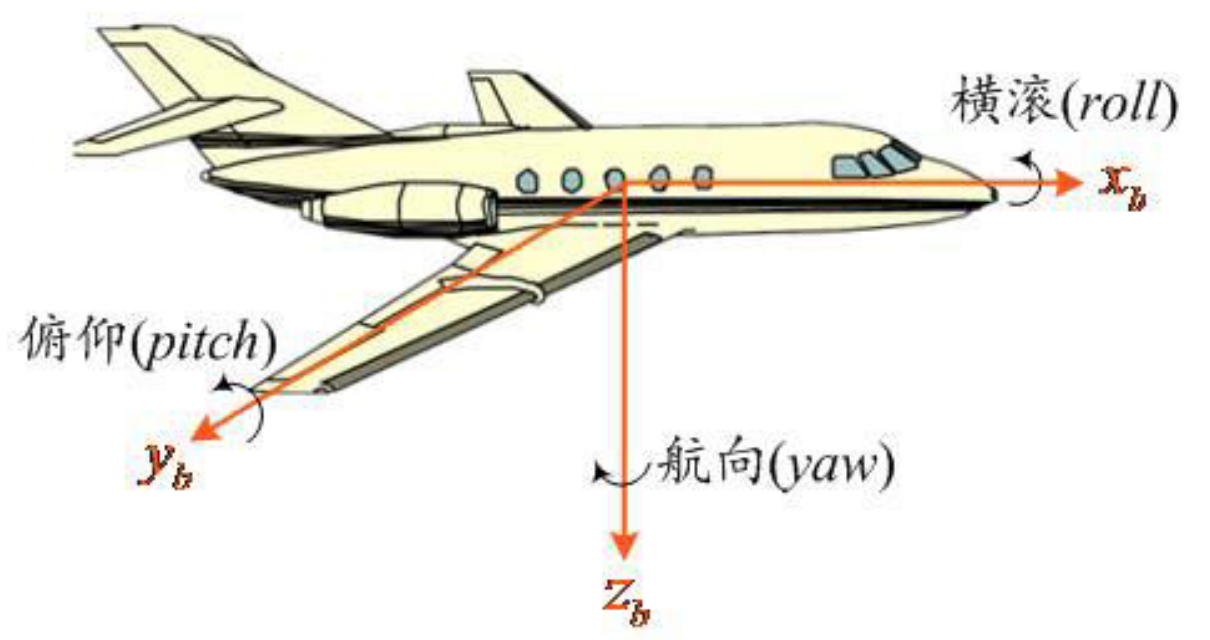
\includegraphics[width=0.65\textwidth]{guide_body_axes.png}
\caption{载体坐标轴及姿态角（假设IMU与载体各轴对齐）}\label{fig:bodyaxes}
\end{figure}
图\ref{fig:bodyaxes}以飞机说明前、右、下机体系及绕各轴的姿态变化。它明确了横滚、俯仰和航向的物理含义，也说明解释IMU姿态前必须确认传感器与载体的安装关系。

本文取$\psi,\phi\in[-\pi,\pi]$、$\theta\in[-\pi/2,\pi/2]$；航向也可等价归化到$[0,2\pi)$。记$c_\alpha=\cos\alpha$、$s_\alpha=\sin\alpha$，方向余弦矩阵为
\begin{equation}
\matr C_b^n=
\begin{bmatrix}
c_\theta c_\psi&-c_\phi s_\psi+s_\phi s_\theta c_\psi&s_\phi s_\psi+c_\phi s_\theta c_\psi\\
c_\theta s_\psi&c_\phi c_\psi+s_\phi s_\theta s_\psi&-s_\phi c_\psi+c_\phi s_\theta s_\psi\\
-s_\theta&s_\phi c_\theta&c_\phi c_\theta
\end{bmatrix},\quad
\matr C_n^b=(\matr C_b^n)^T.
\label{eq:eulermatrix}\end{equation}

$Z$轴比力约为$-g$，与$Z$轴大致朝下相符。本次取$\matr C_s^b=\matr I$，记录设备XYZ相对NED的姿态，并将其作为本次载体坐标系。

“右、前、上”到“前、右、下”的转换仅在原设备确属此安装方式时使用：
\begin{equation}
\matr C_s^b=\begin{bmatrix}0&1&0\\1&0&0\\0&0&-1\end{bmatrix},\quad
\matr f^b=\matr C_s^b\matr f^s,\quad\matr\omega^b=\matr C_s^b\matr\omega^s.
\label{eq:axismatrix}
\end{equation}
其分量形式为
\begin{equation}
\begin{aligned}
f_x^b&=f_y^s,& f_y^b&=f_x^s,& f_z^b&=-f_z^s,\\
\omega_x^b&=\omega_y^s,& \omega_y^b&=\omega_x^s,& \omega_z^b&=-\omega_z^s.
\end{aligned}
\label{eq:axiscomponents}\end{equation}

\subsubsection{双矢量定姿}
地面静止，忽略传感器误差时，
\begin{equation}
\matr g^n=\begin{bmatrix}0\\0\\g\end{bmatrix},\quad
\matr\omega_{ie}^n=\begin{bmatrix}\Omega\cos L\\0\\-\Omega\sin L\end{bmatrix},\quad
\matr g^b=-\overline{\matr f}^b.
\label{eq:referencevectors}
\end{equation}
其中$\matr\omega_{ie}^b=\matr\omega_{ib}^b\approx\overline{\matr\omega}^b$，静止时由陀螺观测获得；$\matr g^b=[-\overline f_x,-\overline f_y,-\overline f_z]^T$。静态比力与重力方向相反，不能把二者视为同向矢量。

两参考矢量在导航系与机体系间的投影关系为：
\begin{equation}
\matr g^b=\matr C_n^b\matr g^n,\qquad
\matr\omega_{ie}^b=\matr C_n^b\matr\omega_{ie}^n.
\label{eq:vectorprojection}\end{equation}
通过叉乘构造第三向量：
\begin{equation}
\matr v=\matr g\times\matr\omega_{ie},\quad
\matr v^b=\matr g^b\times\matr\omega_{ie}^b,\quad
\matr v^n=\matr g^n\times\matr\omega_{ie}^n=\matr C_b^n\matr v^b.
\label{eq:thirdvector}\end{equation}
叉乘的分量及反对称矩阵形式为：
\begin{equation}
\matr a\times\matr b=
\begin{bmatrix}0&-a_z&a_y\\a_z&0&-a_x\\-a_y&a_x&0\end{bmatrix}
\begin{bmatrix}b_x\\b_y\\b_z\end{bmatrix}
=\begin{bmatrix}a_yb_z-a_zb_y\\a_zb_x-a_xb_z\\a_xb_y-a_yb_x\end{bmatrix}.
\end{equation}
将三个投影关系转置后按行排列，定义：
\begin{equation}
\matr R_n=\begin{bmatrix}(\matr g^n)^T\\(\matr\omega_{ie}^n)^T\\(\matr v^n)^T\end{bmatrix},\qquad
\matr R_b=\begin{bmatrix}(\matr g^b)^T\\(\matr\omega_{ie}^b)^T\\(\matr v^b)^T\end{bmatrix},\qquad
\matr R_b=\matr R_n\matr C_b^n.
\end{equation}
因此方向余弦矩阵可写为：
\begin{equation}
\matr C_b^n=\matr R_n^{-1}\matr R_b.
\label{eq:directtriad}\end{equation}
由于$\matr v^n=[0,g\Omega\cos L,0]^T$，导航系参考矩阵及其逆为：
\begin{equation}
\matr R_n=\begin{bmatrix}
0&0&g\\\Omega\cos L&0&-\Omega\sin L\\0&g\Omega\cos L&0
\end{bmatrix},\qquad
\matr R_n^{-1}=\begin{bmatrix}
\tan L/g&1/(\Omega\cos L)&0\\
0&0&1/(g\Omega\cos L)\\1/g&0&0
\end{bmatrix}.
\label{eq:referenceinverse}\end{equation}
代入参考矩阵的逆，得到显式解：
\begin{equation}
\matr C_b^n=
\begin{bmatrix}
\dfrac{\tan L}{g}(\matr g^b)^T+\dfrac{1}{\Omega\cos L}(\matr\omega_{ie}^b)^T\\[4pt]
\dfrac{1}{g\Omega\cos L}(\matr g^b\times\matr\omega_{ie}^b)^T\\[4pt]
\dfrac{1}{g}(\matr g^b)^T
\end{bmatrix}.
\label{eq:directexplicit}\end{equation}
当$g\ne0$且$\Omega\cos L\ne0$时两参考矢量不共线，矩阵可逆。带误差观测直接代入所得矩阵通常不严格正交，因此实际计算采用下一节的正交化形式。

\subsubsection{正交化与姿态角反解}
分别构造导航系与机体系的单位正交基：
\begin{equation}
\begin{aligned}
\matr v_g&=\frac{\matr g^n}{\|\matr g^n\|},&
\matr v_\omega&=\frac{\matr g^n\times\matr\omega_{ie}^n}{\|\matr g^n\times\matr\omega_{ie}^n\|},&
\matr v_{g\omega}&=\frac{(\matr g^n\times\matr\omega_{ie}^n)\times\matr g^n}{\|(\matr g^n\times\matr\omega_{ie}^n)\times\matr g^n\|},\\
\matr w_g&=\frac{\widetilde{\matr g}^b}{\|\widetilde{\matr g}^b\|},&
\matr w_\omega&=\frac{\widetilde{\matr g}^b\times\widetilde{\matr\omega}_{ie}^b}{\|\widetilde{\matr g}^b\times\widetilde{\matr\omega}_{ie}^b\|},&
\matr w_{g\omega}&=\frac{(\widetilde{\matr g}^b\times\widetilde{\matr\omega}_{ie}^b)\times\widetilde{\matr g}^b}{\|(\widetilde{\matr g}^b\times\widetilde{\matr\omega}_{ie}^b)\times\widetilde{\matr g}^b\|}.
\end{aligned}
\label{eq:bothbases}\end{equation}
这里$\widetilde{\matr g}^b=-\overline{\matr f}^b$，$\widetilde{\matr\omega}_{ie}^b=\overline{\matr\omega}^b$；括号明确了连续叉乘的运算顺序。由两组正交基得到：
\begin{equation}
\matr C_b^n=
\begin{bmatrix}\matr v_g^T\\\matr v_\omega^T\\\matr v_{g\omega}^T\end{bmatrix}^{-1}
\begin{bmatrix}\matr w_g^T\\\matr w_\omega^T\\\matr w_{g\omega}^T\end{bmatrix}
=[\matr v_g,\matr v_\omega,\matr v_{g\omega}]
\begin{bmatrix}\matr w_g^T\\\matr w_\omega^T\\\matr w_{g\omega}^T\end{bmatrix}.
\label{eq:orthotriad}\end{equation}
在NED中三基向量依次为地、东、北，因此机体系计算可简写为：
\begin{equation}
\matr d^b=\frac{\matr g^b}{\|\matr g^b\|},\qquad
\matr e^b=\frac{\matr g^b\times\overline{\matr\omega}^b}{\|\matr g^b\times\overline{\matr\omega}^b\|},\qquad
\matr n^b=\matr e^b\times\matr d^b.
\label{eq:triad}\end{equation}
三个矢量分别表示地、东、北方向在机体系中的分量，因此：
\begin{equation}
\matr C_b^n=\begin{bmatrix}(\matr n^b)^T\\(\matr e^b)^T\\(\matr d^b)^T\end{bmatrix}.
\end{equation}
与分别构造两坐标系正交基后计算$\matr V\matr W^T$等价。要求重力模长和叉乘模长非零，检验$\matr C_b^n(\matr C_b^n)^T=\matr I$及$\det\matr C_b^n=1$。

欧拉角按下式提取：
\begin{equation}
\begin{aligned}
\psi&=\operatorname{atan2}(C_{21},C_{11}),\\
\theta&=\operatorname{atan2}(-C_{31},\sqrt{C_{32}^2+C_{33}^2}),\\
\phi&=\operatorname{atan2}(C_{32},C_{33}).
\end{aligned}\label{eq:euler}\end{equation}
当$\theta=\pm\pi/2$时欧拉角出现奇异，航向和横滚不能独立唯一确定，但方向余弦矩阵仍可使用。


\subsection{静态平均时长与噪声抑制}
设每个样本的零均值独立白噪声为$\eta_k$、标准差为$\sigma_\eta$，则平均噪声的RMS为：
\begin{equation}
\overline\eta=\frac1N\sum_{k=1}^N\eta_k,\qquad
\operatorname{RMS}(\overline\eta)=\sqrt{\mathrm E[\overline\eta^2]}
=\frac{\sigma_\eta}{\sqrt N}=\frac{\mathrm{ARW}}{\sqrt T},\qquad T=N\Delta t.
\label{eq:noiseaverage}\end{equation}
ARW与$T$须使用一致的时间单位。
若ARW系数为$N_g$，单位$^\circ/\sqrt{\mathrm h}$，独立白噪声条件下：
\begin{equation}
\sigma_{\overline\omega}(T_h)=\frac{N_g}{\sqrt{T_h}}\quad(^\circ/\mathrm h),\qquad T_h=T_s/3600.
\end{equation}
平均噪声小于零偏量级三分之一，需：
\begin{equation}
\frac{N_g}{\sqrt{T_h}}\le\frac{|b_g|}{3}
\quad\Longrightarrow\quad T_h\ge\left(\frac{3N_g}{|b_g|}\right)^2,\qquad
T_s\ge3600\left(\frac{3N_g}{|b_g|}\right)^2.
\label{eq:averagetime}
\end{equation}
若加速度计VRW为$N_a$，单位$(\mathrm{m/s})/\sqrt{\mathrm h}$，则换成秒制后$N_{a,s}=N_a/60$，对$b_a$以m/s$^2$表达时有：
\begin{equation}
\sigma_{\overline f}(T_s)=\frac{N_a}{60\sqrt{T_s}}\quad(\mathrm{m/s^2}),\qquad
T_s\ge\left(\frac{3N_a}{60|b_a|}\right)^2.
\end{equation}
以IMU-100C的名义参数$N_g=0.005^\circ/\sqrt{\mathrm h}$、$b_g=0.05^\circ$/h估算，需0.09~h即324~s。加速度计VRW与零偏比较也必须统一时间及加速度单位。
